\title{Counters}
\begin{document}
\section{Types of Counters}

\begin{frame}{What is a counter?}
  \begin{definition}
    A \alert{counter} is a clock sequential circuit whose state diagram is a single cycle.
  \end{definition}
  \begin{itemize}
    \item A counter with m states is called a \alert{modulo-m counter} or a \alert{divide-by-m counter}.
    \item An \alert{n-bit binary counter} has n flip-flops and $2^n$ states, visited in sequence.
  \end{itemize}
\end{frame}

\subsection{Ripple Counters}

\begin{frame}{Ripple counter}
  A ripple counter uses n T flip-flops and a clock signal.
  \begin{center}
    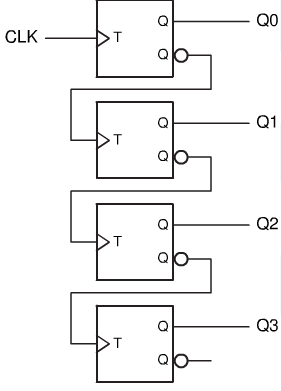
\includegraphics[scale=0.3]{RippleCounterLogic}
  \end{center}
  What is one drawback of a ripple counter?
\end{frame}

\subsection{Synchronous Counters}

\begin{frame}{Synchronous serial counter}
  \begin{center}
    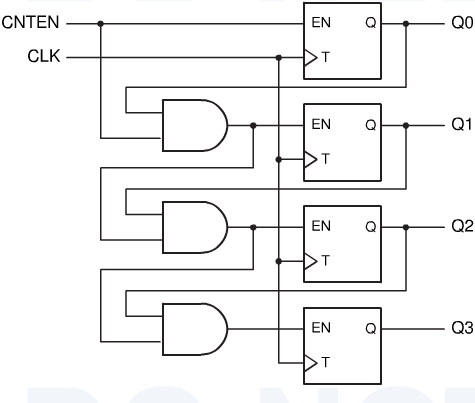
\includegraphics[scale=0.5]{SynchronousSerialCounter}
  \end{center}
\end{frame}

\begin{frame}{Synchronous parallel counter}
  \begin{center}
    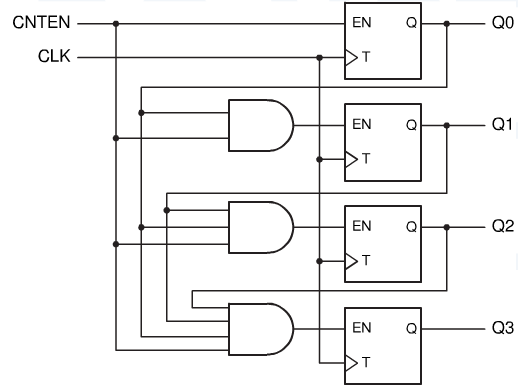
\includegraphics[scale=0.5]{SynchronousParallelCounter}
  \end{center}
\end{frame}

\section{MSI Counters}
\subsection{74x163 Counter}

\begin{frame}{MSI 74x163 counter}
  \begin{center}
    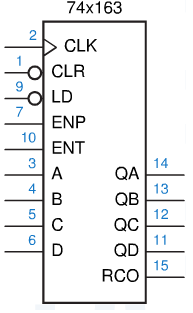
\includegraphics[scale=0.5]{74x163Schematic}
  \end{center}
\end{frame}

\begin{frame}{Possible 74x163 implementation}
  \begin{center}
    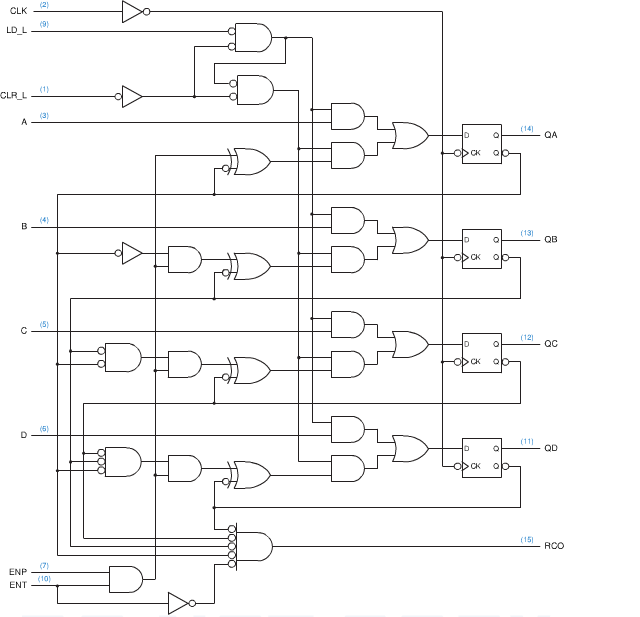
\includegraphics[scale=0.3]{Wakerly_Figure_8_28}
  \end{center}
\end{frame}

\begin{frame}{Free-running 74x163 configuration}
  \begin{center}
    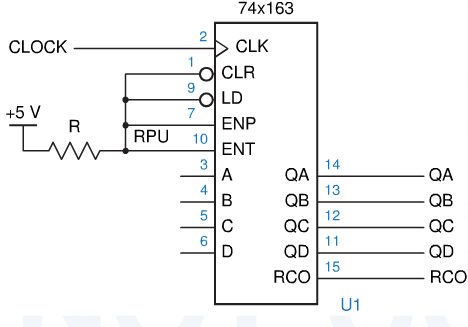
\includegraphics[scale=0.4]{74x163SchematicFreeRunning}
  \end{center}
  A free running counter can be used to divide by powers of two, since each of the four outputs has half the frequency of the previous output.
\end{frame}

\subsection{74x169 Counter}

\begin{frame}{MSI 74x169 counter}
  \begin{center}
    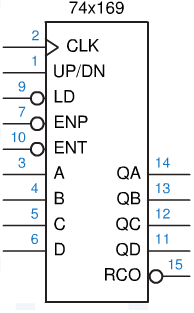
\includegraphics[scale=0.5]{74x169Schematic}
  \end{center}
\end{frame}

\section{Decoding Binary Counter States}

\begin{frame}{How can we select a device based on the counter?}
  \begin{center}
    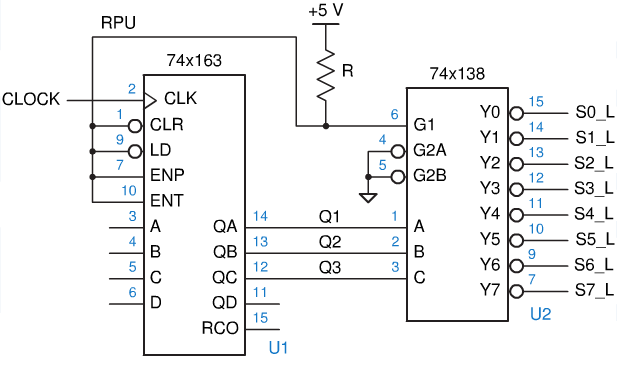
\includegraphics[scale=0.5]{CounterDecoder}
  \end{center}
  What is a possible problem with this implementation?
\end{frame}

\begin{frame}{Handling the problem}
  \begin{center}
    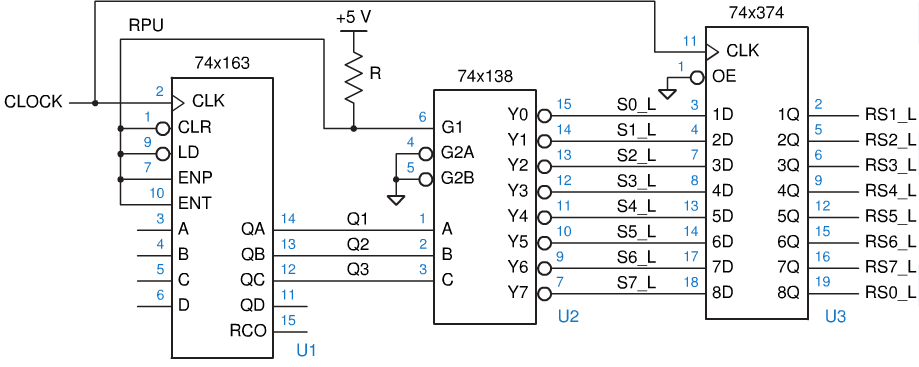
\includegraphics[scale=0.35]{CounterDecoderRegister}
  \end{center}
\end{frame}

\end{document}
